\chapter{La reproduction sexuée des mammifères}\label{ch:b2:mammal-reproduction}

Un ovocyte humain mesure un dixième de millimètre de diamètre~: c'est la
plus grande cellule du corps~; un spermatozoïde est un noyau muni d'une
hélice, l'un de trois cents millions libérés en même temps, dont
quelques dizaines atteindront l'ovocyte et un seul y entrera. En une
semaine, l'œuf fécondé est devenu une sphère creuse qui s'enfouit dans
la paroi de l'utérus et construit, à partir de ses propres cellules
externes, un organe --- le \omterm{def:b2:mammal-reproduction:placenta}{placenta} --- par lequel sa mère le nourrira
pendant neuf mois. Puis il naît et se nourrit de lait. Tous les
mammifères font cela~; aucun autre animal ne fait tout cela. Ce chapitre
suit les gamètes jusqu'à la fécondation, l'embryon jusqu'à la \omterm{def:b2:mammal-reproduction:implantation}{nidation},
et l'organisme au fil de la gestation, de la naissance et de la
lactation, et se termine sur la façon dont se construisent les deux
sexes.

\section{Gonades et gamètes}

\begin{definition}[Le testicule et la spermatogenèse]\label{def:b2:mammal-reproduction:testis}
\index{spermatogenese@spermatogenèse}\index{tube seminifere@tube séminifère}\index{cellule de Sertoli}\index{cellule de Leydig}
Le \emph{testicule} est une masse de \emph{tubes séminifères}, longs de
plusieurs centaines de mètres au total, dont les parois produisent les
spermatozoïdes~; entre les tubes se trouvent les \emph{cellules de
Leydig}, qui produisent la testostérone. Dans la paroi du tube, les
\emph{spermatogonies} situées à la périphérie se divisent par mitose,
entretenant une population souche et envoyant des cellules vers
l'intérieur~; celles-ci grossissent en \emph{spermatocytes} primaires,
qui subissent la \omterm{def:b2:meiosis-heredity:meiosis}{méiose} I (et donnent deux spermatocytes secondaires)
puis la \omterm{def:b2:meiosis-heredity:meiosis}{méiose} II (et donnent quatre \emph{spermatides} \omterm{def:b2:meiosis-heredity:meiosis}{haploïdes})~; les
spermatides perdent la plus grande partie de leur cytoplasme,
condensent leur noyau, développent un flagelle et coiffent le noyau de
l'\emph{acrosome}, une vésicule d'enzymes, pour devenir des
\emph{spermatozoïdes} libérés dans la lumière. De grandes
\emph{cellules de Sertoli} traversent la paroi, nourrissent les
cellules germinales et forment, par les jonctions serrées qui les
unissent, une \emph{barrière hémato-testiculaire} qui tient le système
immunitaire à l'écart de cellules apparues seulement à la puberté. La
séquence entière dure environ \num{64} jours chez l'homme et fournit
quelque $10^{8}$ spermatozoïdes par jour, de la puberté à la
vieillesse. Les spermatozoïdes quittent le testicule immobiles et
mûrissent pendant deux semaines dans l'\emph{épididyme}.
\end{definition}

\begin{omfigure}
\begin{tikzpicture}[every node/.style={font=\scriptsize}]
  % tubule cross-section: concentric layers
  \draw[thick, fill=omExo!15] (0,0) circle (2.5);
  \draw[thick, fill=omExo!8] (0,0) circle (2.2);
  \draw[thick, fill=omDef!10] (0,0) circle (1.6);
  \draw[thick, fill=omProp!12] (0,0) circle (1.0);
  \draw[thick, fill=white] (0,0) circle (0.45);
  % cells
  \foreach \a in {0,30,...,330} \draw[thick, fill=omDef!40] (\a:2.0) circle (0.13);
  \foreach \a in {15,45,...,345} \draw[thick, fill=omDef!70] (\a:1.32) circle (0.16);
  \foreach \a in {0,20,...,340} \draw[thick, fill=omProp!60] (\a:0.75) circle (0.08);
  \foreach \a in {10,40,...,340} \draw[thick, omProp!80!black] (\a:0.45) -- (\a:0.15);
  % Sertoli cell: tall wedge
  \draw[thick, omExo!70!black, fill=omExo!40, opacity=0.6] (100:2.2) .. controls (90:1.6) and (95:0.9) .. (92:0.5) .. controls (80:0.9) and (75:1.6) .. (72:2.2) -- cycle;
  % Leydig cells outside
  \foreach \p in {(2.9,0.8),(3.1,0.3),(2.8,-0.3)} \draw[thick, fill=omThm!40] \p circle (0.14);
  % labels
  \draw (2.0,0) -- (3.6,-0.5) node[right, align=left] {spermatogonies ($2n$)\\à la périphérie};
  \draw (1.32,-0.7) -- (3.6,-1.5) node[right, align=left] {spermatocytes primaires\\(méiose I)};
  \draw (0.75,-0.4) -- (3.6,-2.4) node[right, align=left] {spermatides ($n$)};
  \draw (0.3,-0.2) -- (3.6,-3.1) node[right, align=left] {spermatozoïdes dans la lumière};
  \draw (2.95,0.55) -- (3.6,0.6) node[right, align=left] {cellules de Leydig~:\\testostérone};
  \draw (88:1.4) -- (3.6,1.8) node[right, align=left] {cellule de Sertoli traversant la paroi};
  \node[anchor=east, align=right] at (-2.7,0) {extérieur\\(lame basale)};
\end{tikzpicture}

{\small Un \omterm{def:b2:mammal-reproduction:testis}{tube séminifère} en coupe transversale. Les cellules
germinales mûrissent de la paroi externe (spermatogonies) vers
l'intérieur (spermatocytes, spermatides, spermatozoïdes dans la
lumière), soutenues par les \omterm{def:b2:mammal-reproduction:testis}{cellules de Sertoli}~; les \omterm{def:b2:mammal-reproduction:testis}{cellules de
Leydig}, entre les tubes, produisent la testostérone.}
\end{omfigure}

\begin{omfigure}
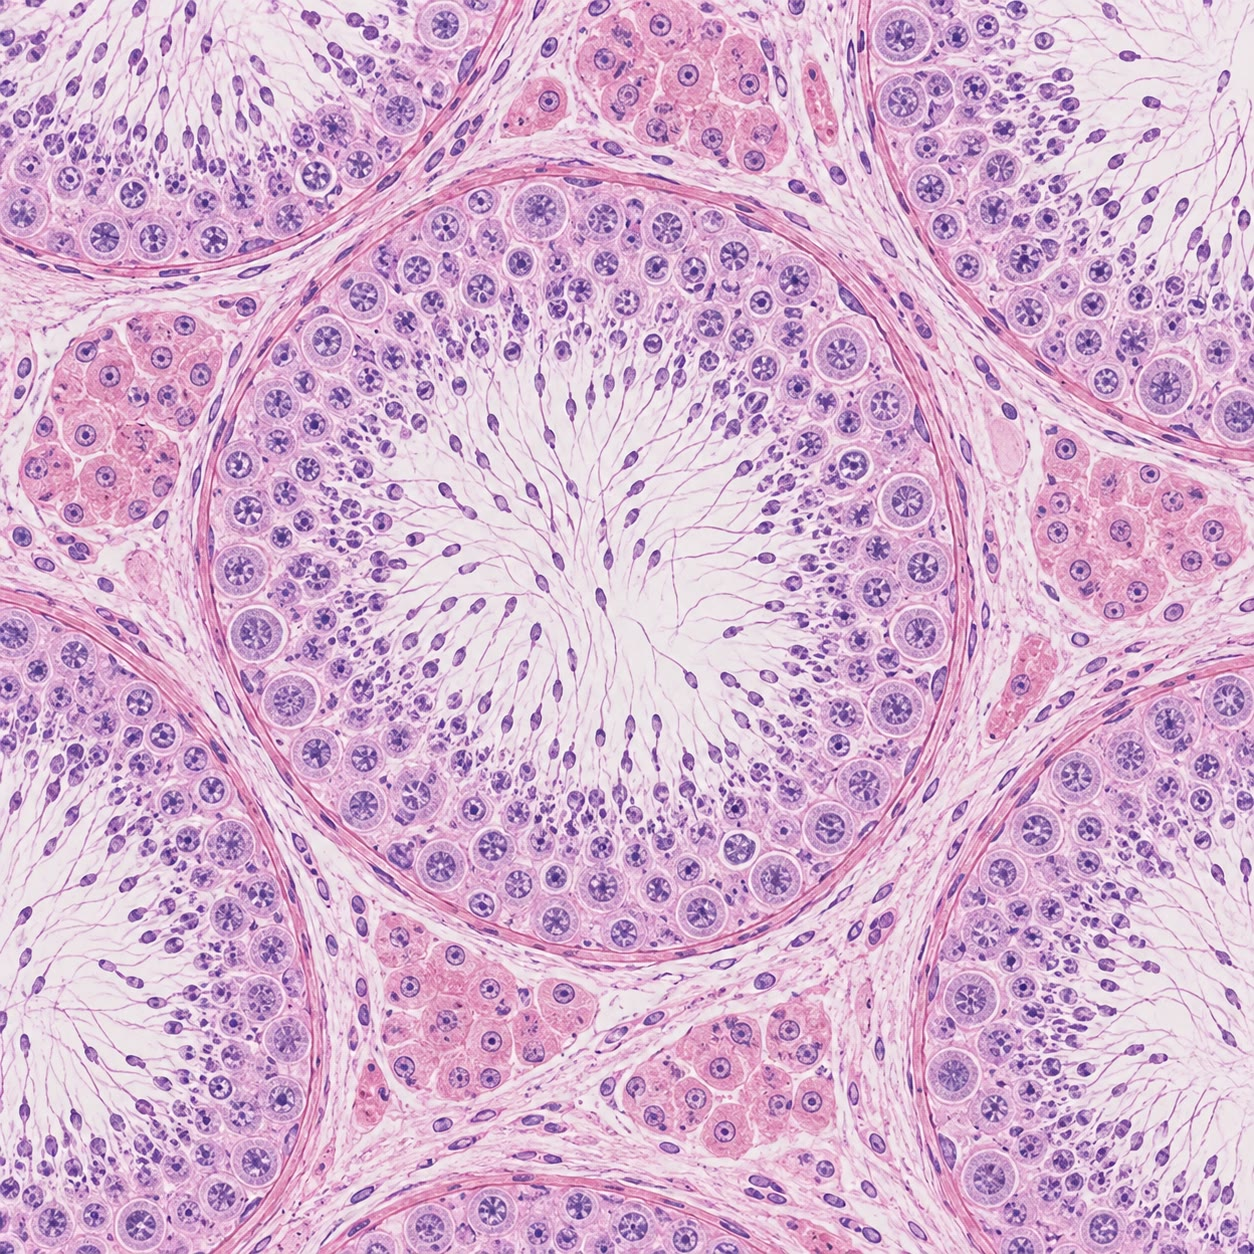
\includegraphics[width=0.42\linewidth]{images/book4/ai/b4-08-testis-histology.jpg}\hspace{0.04\linewidth}
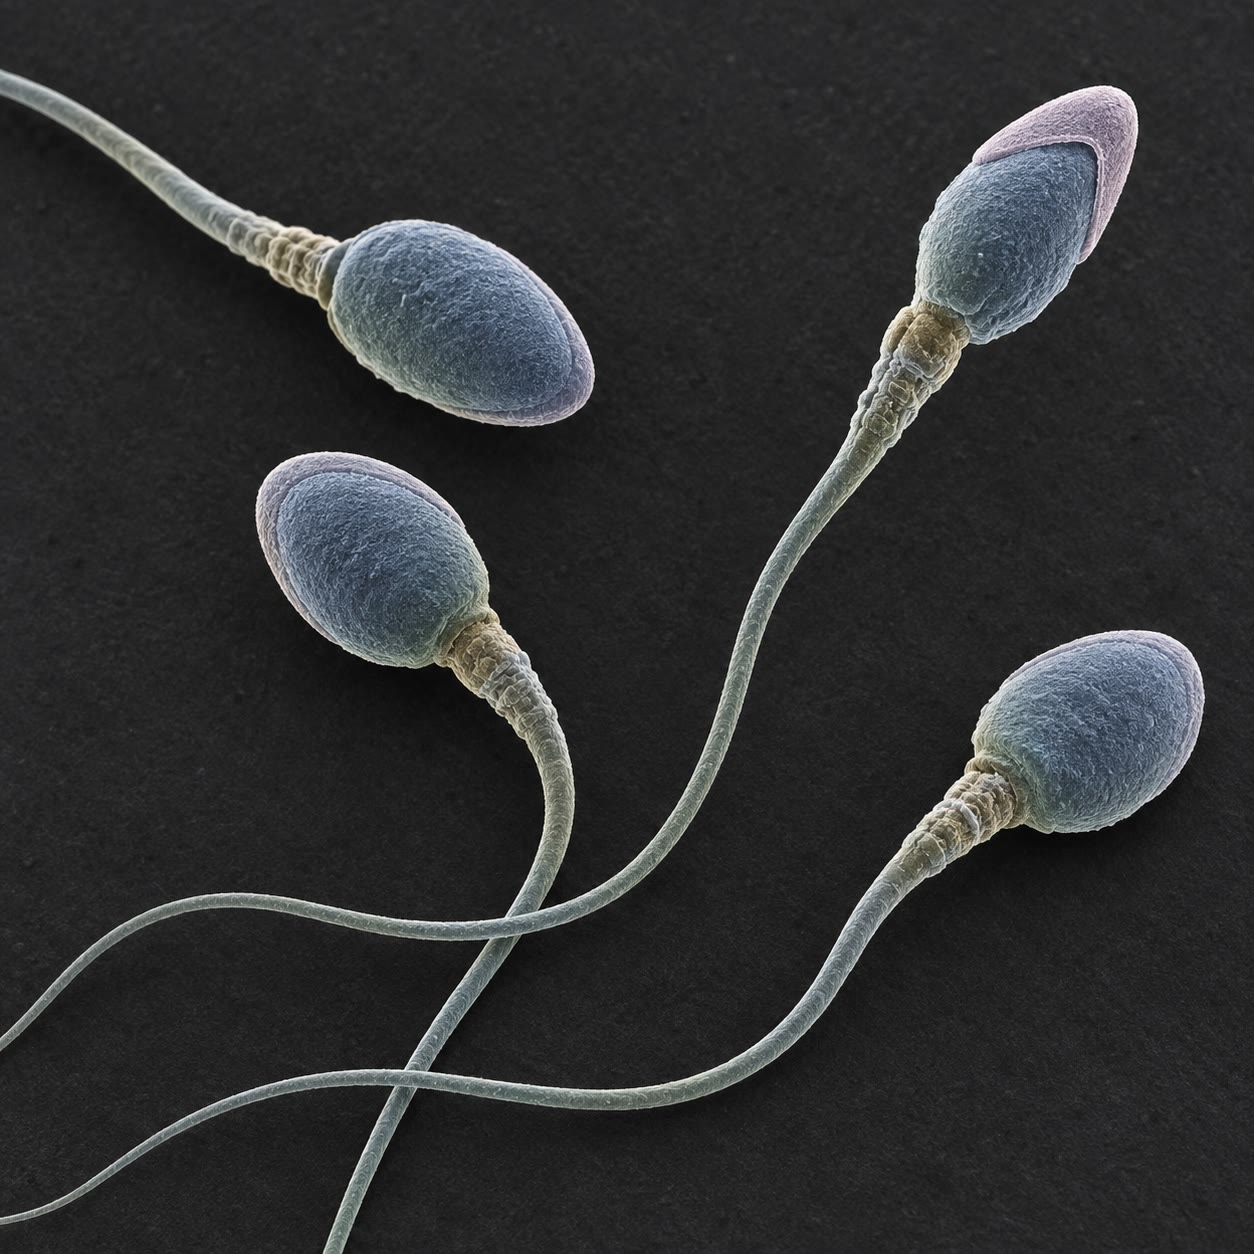
\includegraphics[width=0.42\linewidth]{images/book4/ai/b4-08-sperm-sem.jpg}

{\small À gauche~: \omterm{def:b2:mammal-reproduction:testis}{tubes séminifères} en coupe, les cellules germinales
étagées de la paroi à la lumière. À droite~: spermatozoïdes au
microscope électronique à balayage, la coiffe acrosomique visible sur
les têtes.}
\end{omfigure}

\begin{definition}[L'ovaire et l'ovogenèse]\label{def:b2:mammal-reproduction:ovary}
\index{ovogenese@ovogenèse}\index{follicule}\index{ovulation}\index{corps jaune}
L'ovogenèse est presque en tout point l'image inversée de la
\omterm{def:b2:mammal-reproduction:testis}{spermatogenèse}. Les \emph{ovogonies} ne se multiplient que chez le
fœtus~: à la naissance, une fille possède un stock d'environ un million
d'\emph{ovocytes} primaires, chacun bloqué en \omterm{prop:b2:meiosis-heredity:stages}{prophase I} de \omterm{def:b2:meiosis-heredity:meiosis}{méiose} et
entouré d'une seule couche de cellules --- un \emph{follicule
primordial} --- et il ne s'en forme jamais de nouveaux. À partir de la
puberté, chaque mois, une cohorte de follicules se développe~:
l'ovocyte grossit, les cellules de la \emph{granulosa} qui l'entourent
se multiplient en plusieurs couches, une \emph{thèque} externe se
forme, une cavité remplie de liquide s'ouvre (le \emph{follicule de De
Graaf}, de deux centimètres de diamètre), et en général un seul atteint
l'\emph{ovulation}~: l'ovocyte, qui achève seulement alors la \omterm{def:b2:meiosis-heredity:meiosis}{méiose} I et
se bloque de nouveau en métaphase II, est expulsé dans l'oviducte avec
sa couronne de cellules de la granulosa. Le follicule vidé devient le
\emph{corps jaune}, une glande temporaire qui sécrète la progestérone.
La \omterm{def:b2:meiosis-heredity:meiosis}{méiose} produit un ovocyte et trois minuscules globules polaires ---
tout le cytoplasme va à une seule cellule --- et la \omterm{def:b2:meiosis-heredity:meiosis}{méiose} II ne
s'achève que si un spermatozoïde entre. Sur le million d'ovocytes,
environ \num{400} sont ovulés au cours d'une vie~; les autres
dégénèrent (\emph{atrésie}), et lorsque le stock est épuisé, vers
cinquante ans, les cycles s'arrêtent~: c'est la ménopause.
\end{definition}

\begin{omfigure}
\begin{tikzpicture}[every node/.style={font=\scriptsize}, >=stealth]
  % timeline of oogenesis vs spermatogenesis
  \draw[thick, ->] (0,3.0) -- (12.6,3.0); \node[anchor=west] at (12.6,3.0) {âge};
  \foreach \x/\l in {0/{fœtus}, 2.2/{naissance}, 4.6/{puberté}, 10.2/{$\sim$50 ans}}
    \draw (\x,3.1) -- (\x,2.9) node[above=0.15cm] {\l};
  % oogenesis line
  \node[anchor=east, omThm] at (-0.2,1.5) {ovogenèse};
  \draw[very thick, omThm] (0,1.5) -- (1.6,1.5); \node[above, omThm, align=center] at (0.8,1.55) {les ovogonies\\se multiplient};
  \draw[very thick, omThm, dashed] (1.6,1.5) -- (4.6,1.5); \node[below, omThm] at (3.1,1.45) {blocage en prophase I};
  \draw[very thick, omThm] (4.6,1.5) -- (10.2,1.5); \node[above, omThm, align=center] at (7.4,1.55) {une ovulation par mois~;\\méiose I achevée à l'ovulation, II à la fécondation};
  \fill[omThm] (10.2,1.5) circle (0.07); \node[below, omThm] at (10.2,1.45) {stock épuisé};
  % spermatogenesis line
  \node[anchor=east, omDef] at (-0.2,0.3) {spermatogenèse};
  \draw[very thick, omDef, dashed] (0,0.3) -- (4.6,0.3); \node[above, omDef] at (2.3,0.35) {spermatogonies au repos};
  \draw[very thick, omDef, ->] (4.6,0.3) -- (12.6,0.3); \node[above, omDef] at (8.6,0.35) {continue~: $10^{8}$ par jour, 64 jours chacun, depuis des cellules souches};
\end{tikzpicture}

{\small Les deux gamétogenèses dans le temps. Les ovocytes sont tous
formés avant la naissance et libérés un par un à partir d'un stock
fini~; les spermatozoïdes sont produits en continu à partir de cellules
souches pendant toute la vie adulte.}
\end{omfigure}

\begin{omfigure}
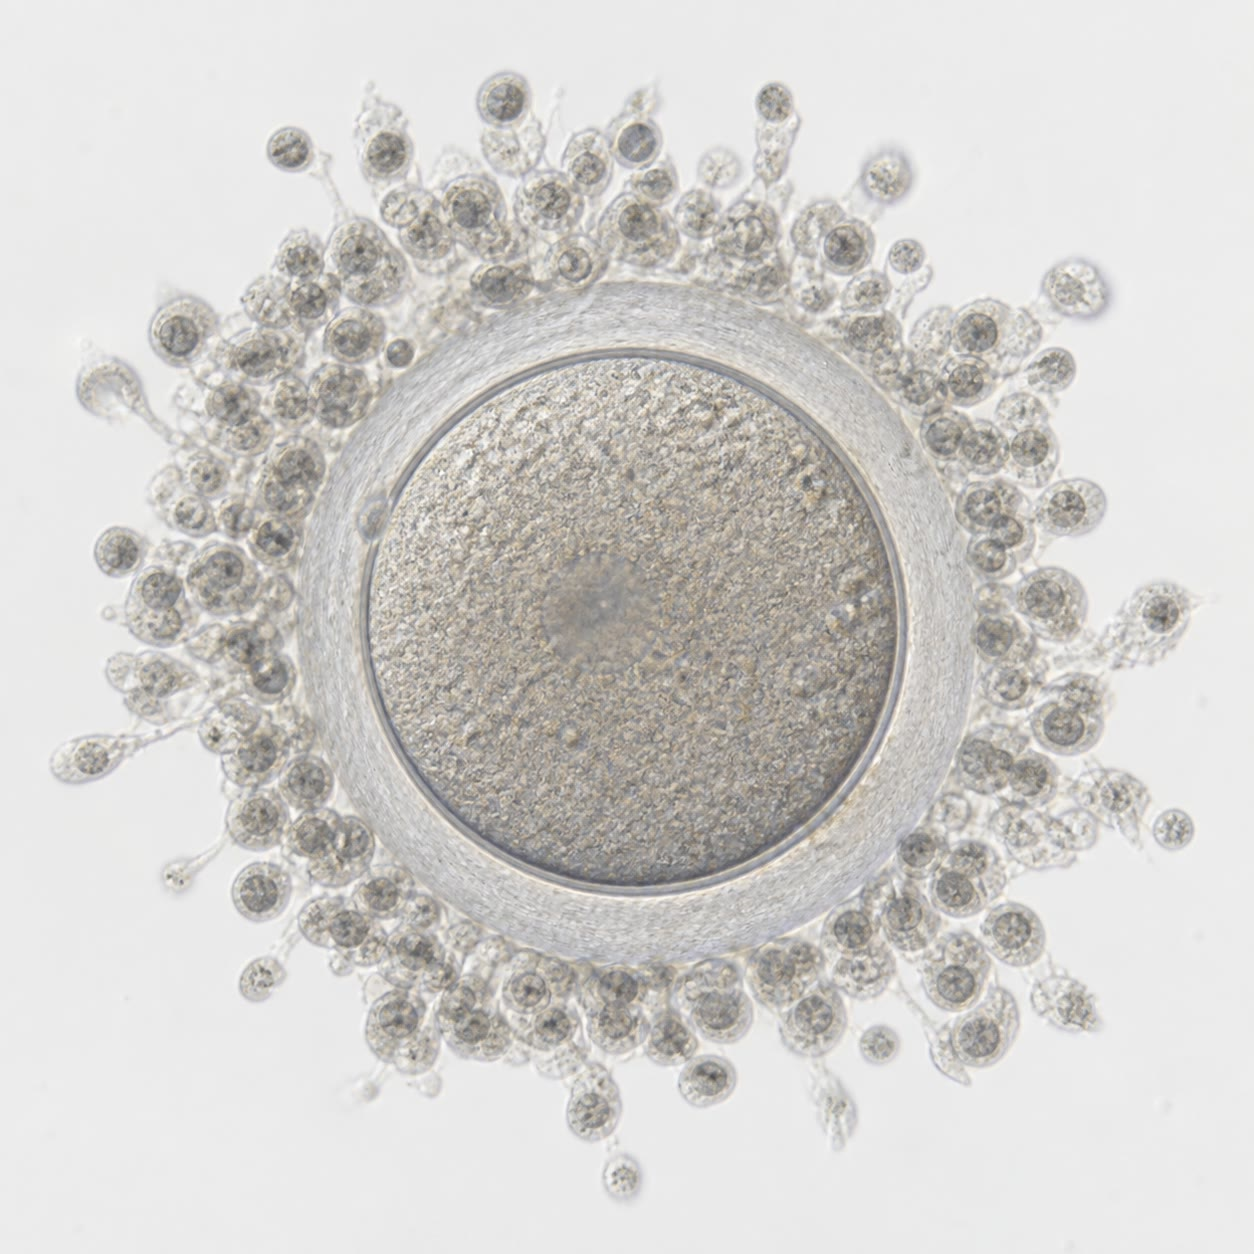
\includegraphics[width=0.46\linewidth]{images/book4/ai/b4-08-oocyte.jpg}

{\small Un ovocyte ovulé~: la cellule, son enveloppe transparente (la
\omterm{prop:b2:mammal-reproduction:fertilisation}{zone pellucide}), et le nuage de cellules de la granulosa qui a quitté le
\omterm{def:b2:mammal-reproduction:ovary}{follicule} avec elle.}
\end{omfigure}

\section{La fécondation}

\begin{proposition}[Les étapes de la fécondation]\label{prop:b2:mammal-reproduction:fertilisation}
\index{fecondation!chez les mammiferes@chez les mammifères}\index{reaction acrosomique@réaction acrosomique}\index{zone pellucide}\index{reaction corticale@réaction corticale}
Les spermatozoïdes déposés dans le vagin --- quelque $3\times 10^{8}$ ---
traversent la glaire cervicale, sont entraînés vers le haut de l'utérus
par ses contractions, et quelques centaines atteignent en une heure
l'ampoule de l'oviducte, où l'ovocyte attend pendant une journée. En
chemin, les spermatozoïdes subissent la \emph{capacitation}~: les
sécrétions des voies génitales femelles débarrassent leurs membranes de
protéines de revêtement et les rendent hyperactifs. Au contact de
l'ovocyte, un spermatozoïde traverse les cellules de la granulosa, se fixe
à une glycoprotéine de la \emph{\omterm{prop:b2:mammal-reproduction:fertilisation}{zone pellucide}} et subit la
\emph{\omterm{prop:b2:mammal-reproduction:fertilisation}{réaction acrosomique}}, qui libère des enzymes creusant un passage
à travers la zone~; sa membrane fusionne avec celle de l'ovocyte, et le
noyau du spermatozoïde entre. L'ovocyte répond en quelques secondes~: une
vague de calcium le parcourt, et des granules corticaux libèrent des
enzymes qui durcissent la zone et en détachent les récepteurs des
spermatozoïdes --- c'est la \emph{\omterm{prop:b2:mammal-reproduction:fertilisation}{réaction corticale}}, le blocage de la
polyspermie. L'ovocyte achève la \omterm{def:b2:meiosis-heredity:meiosis}{méiose} II, expulse le second globule
polaire, et les deux \emph{pronucléus} \omterm{def:b2:meiosis-heredity:meiosis}{haploïdes} répliquent leur ADN, se
rapprochent et entrent dans la première mitose~: le zygote a un jour. La
spécificité d'espèce réside dans les protéines de la zone, ce qui
explique qu'un spermatozoïde de souris n'entre pas dans un ovocyte humain.
\end{proposition}
\begin{proof}[Faits expérimentaux]
Edwards et Steptoe (1978) fécondèrent dans une boîte, avec des
spermatozoïdes capacités, un ovocyte humain prélevé dans l'ovaire peu
avant l'\omterm{def:b2:mammal-reproduction:ovary}{ovulation}, cultivèrent l'embryon jusqu'au stade huit cellules
et le replacèrent dans l'utérus, où il s'implanta et naquit~: c'était la
fécondation in vitro. Chaque étape de la séquence ci-dessus avait
d'abord été établie chez l'oursin et la souris, où l'on peut observer la
fusion, la vague calcique et la libération des granules corticaux~; chez
la souris, la suppression par \omterm{def:b2:genome-diversification:mutation}{mutation} d'une glycoprotéine de la zone
(ZP2 ou ZP3) donne des ovocytes auxquels les spermatozoïdes ne peuvent
pas se fixer.
\end{proof}

\begin{theorem}[Pourquoi un ovocyte a besoin de millions de spermatozoïdes]\label{thm:b2:mammal-reproduction:poisson}
\index{polyspermie}
Si, sur $N$ spermatozoïdes déposés, chacun atteint la surface de
l'ovocyte indépendamment avec une faible probabilité $\pi$, le nombre de
ceux qui arrivent suit une loi de Poisson de moyenne $m = N\pi$, et la
probabilité qu'au moins un arrive vaut
\[
P = 1 - e^{-m}.
\]
Avec $N = 3\times 10^{8}$ et $\pi \approx 10^{-8}$, $m \approx 3$
et $P \approx 0.95$~; avec $N = 2\times 10^{7}$ (le seuil clinique
d'oligospermie), $m = 0.2$ et $P = 0.18$. La même arithmétique montre
pourquoi le blocage de la polyspermie est indispensable~: lorsque $P$ est
élevée, plusieurs spermatozoïdes arrivent à quelques secondes
d'intervalle, et un ovocyte pénétré par deux d'entre eux serait triploïde
et mourrait.
\end{theorem}
\begin{proof}
Chaque spermatozoïde est une épreuve indépendante de probabilité de
succès $\pi$~; le nombre de succès suit une loi binomiale, qui, pour $N$
grand et $\pi$ petit, est une loi de Poisson de moyenne $N\pi$. La
probabilité d'aucun succès vaut $e^{-m}$, celle d'au moins un
$1 - e^{-m}$~; la probabilité de deux succès ou plus vaut
$1 - e^{-m}(1 + m)$, environ $0.8$ pour
$m = 3$.
\end{proof}

\begin{omfigure}
\begin{tikzpicture}[every node/.style={font=\scriptsize}, >=stealth]
  \foreach \x/\lab in {0/{1. le spermatozoïde\\se fixe à la zone}, 3.3/{2. réaction acrosomique~:\\les enzymes creusent un passage}, 6.6/{3. fusion des membranes~;\\vague calcique}, 9.9/{4. réaction corticale~:\\zone durcie,\\méiose II achevée}} {
    \begin{scope}[xshift=\x cm]
      \draw[thick, fill=omThm!8] (0,0) circle (0.9);
      \draw[thick, omExo!70!black] (0,0) circle (1.15);
      \node[below, align=center] at (0,-1.3) {\lab};
    \end{scope}
  }
  % stage 1: sperm at zona
  \draw[thick, fill=omDef!50] (-1.45,0.1) ellipse (0.18 and 0.11); \draw[thick, omDef] (-1.63,0.1) .. controls (-2.0,0.4) and (-2.2,-0.2) .. (-2.5,0.1);
  % stage 2: sperm digging through zona
  \begin{scope}[xshift=3.3cm]
    \fill[white] (-1.2,0.0) circle (0.12);
    \draw[thick, fill=omDef!50] (-1.05,0.05) ellipse (0.18 and 0.11); \draw[thick, omDef] (-1.23,0.05) .. controls (-1.6,0.35) and (-1.8,-0.25) .. (-2.1,0.05);
    \foreach \a in {150,170,190,210} \draw[omProp, thick] (-1.2,0.0) -- ++(\a:0.25);
  \end{scope}
  % stage 3: fused, calcium wave
  \begin{scope}[xshift=6.6cm]
    \fill[white] (-1.15,0.0) circle (0.12);
    \draw[thick, fill=omDef!50] (-0.75,0.0) ellipse (0.18 and 0.11);
    \draw[thick, omDef] (-0.93,0.0) .. controls (-1.3,0.3) and (-1.5,-0.3) .. (-1.8,0.0);
    \foreach \r in {0.35,0.55,0.75} \draw[omProp, thick] (-0.75,0) ++(-60:\r) arc (-60:60:\r);
  \end{scope}
  % stage 4: hardened zona, polar body, pronuclei
  \begin{scope}[xshift=9.9cm]
    \draw[very thick, omExo!70!black] (0,0) circle (1.15);
    \draw[thick, fill=omDef!30] (-0.25,0.05) circle (0.2); \draw[thick, fill=omThm!30] (0.25,0.05) circle (0.2);
    \draw[thick, fill=omThm!20] (0.55,0.95) circle (0.12);
    \node[anchor=west] at (1.2,0.9) {globule polaire};
    \draw (0.45,0.05) -- (1.2,-0.35); \node[anchor=west] at (1.2,-0.35) {deux pronucléus};
  \end{scope}
\end{tikzpicture}

{\small La fécondation en quatre étapes~: fixation à la zone, \omterm{prop:b2:mammal-reproduction:fertilisation}{réaction
acrosomique}, fusion et vague calcique, et \omterm{prop:b2:mammal-reproduction:fertilisation}{réaction corticale} qui ferme
l'ovocyte aux autres spermatozoïdes pendant qu'il achève sa \omterm{def:b2:meiosis-heredity:meiosis}{méiose}.}
\end{omfigure}

\section{La nidation et le placenta}

\begin{definition}[Segmentation, blastocyste, nidation]\label{def:b2:mammal-reproduction:implantation}
\index{blastocyste}\index{trophoblaste}\index{masse cellulaire interne}\index{nidation}
Le zygote se divise toutes les douze à vingt heures sans croître (c'est
la \emph{segmentation}) tandis qu'il descend l'oviducte~: deux cellules,
quatre, huit, une boule compacte de seize (la \emph{morula}), et au
cinquième jour un \emph{blastocyste} d'une centaine de cellules~: une
couche externe, le \emph{trophoblaste}, autour d'une cavité, avec un
amas de cellules d'un côté, la \emph{masse cellulaire interne}. Le
trophoblaste construira le \omterm{def:b2:mammal-reproduction:placenta}{placenta} et les annexes~; la masse cellulaire
interne deviendra l'embryon --- et, prélevée à ce stade, fournit des
cellules souches embryonnaires. Au sixième jour, le blastocyste
s'échappe de sa \omterm{prop:b2:mammal-reproduction:fertilisation}{zone pellucide}, adhère à la muqueuse utérine, et le
trophoblaste l'envahit~: des cellules fusionnent en un front
plurinucléé qui digère le tissu maternel et ouvre des capillaires
maternels, si bien qu'au douzième jour l'embryon est enfoui dans la
paroi et baigné de sang maternel. C'est la \emph{nidation}. Elle ne
réussit que dans un utérus préparé par la progestérone, pendant une
fenêtre de quelques jours~; environ la moitié des conceptions humaines
échouent avant cette étape ou à ce moment, le plus souvent à cause
d'erreurs chromosomiques de l'ovocyte.
\end{definition}

\begin{omfigure}
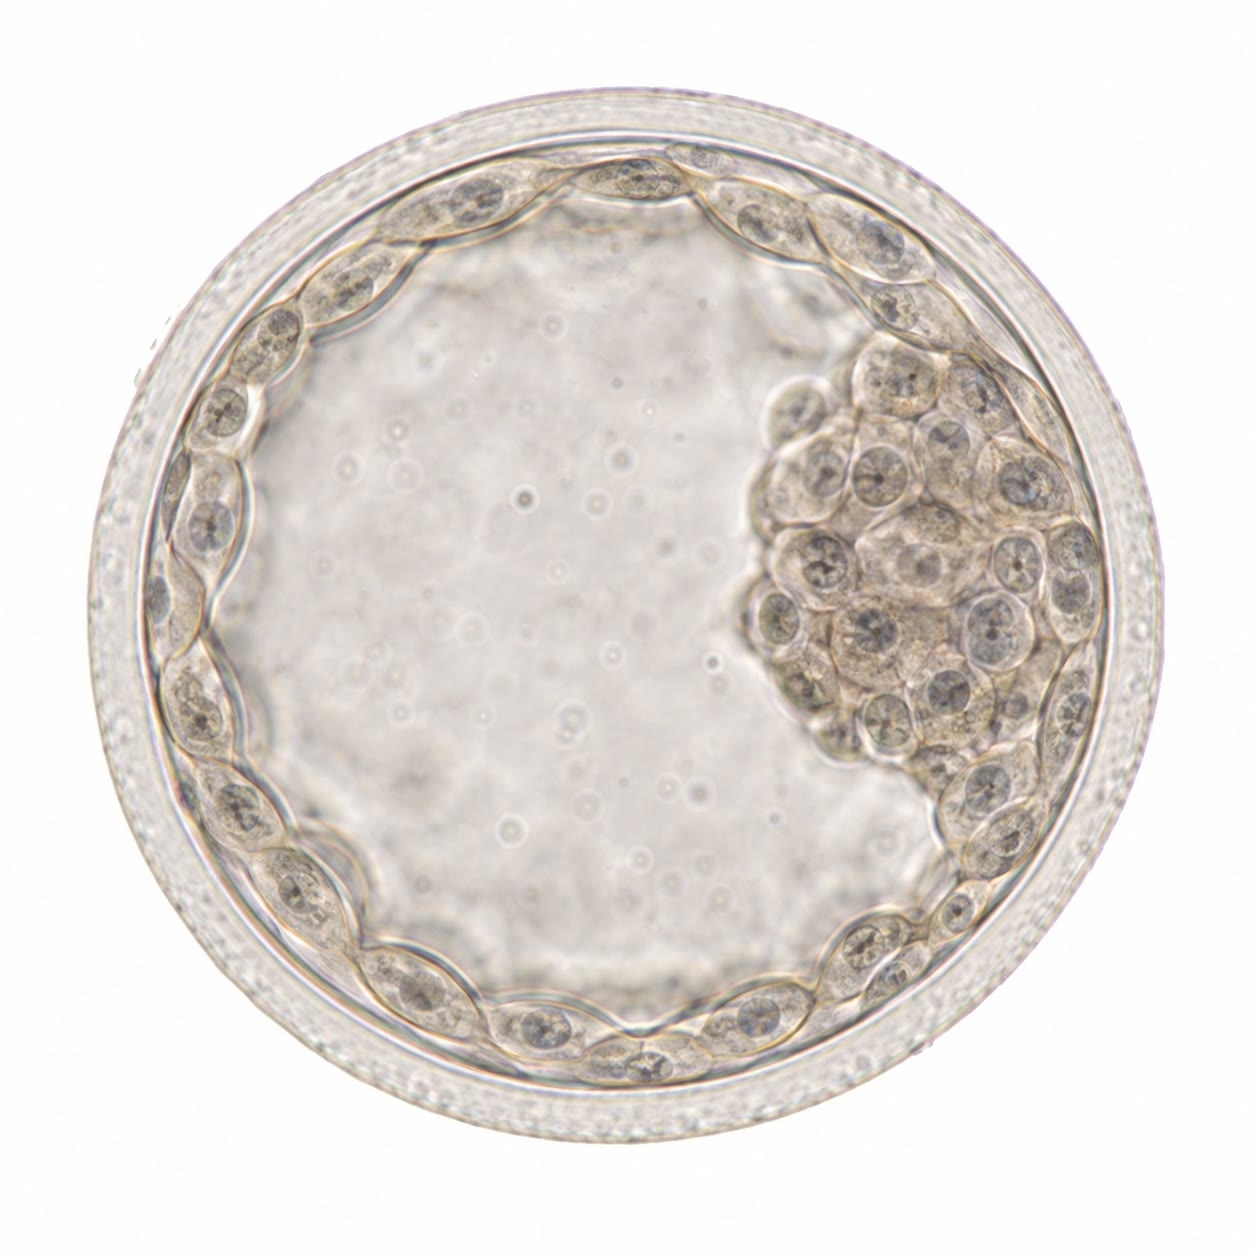
\includegraphics[width=0.42\linewidth]{images/book4/ai/b4-08-blastocyst.jpg}

{\small Un \omterm{def:b2:mammal-reproduction:implantation}{blastocyste} au cinquième jour~: le \omterm{def:b2:mammal-reproduction:implantation}{trophoblaste} externe autour
de la cavité, et la \omterm{def:b2:mammal-reproduction:implantation}{masse cellulaire interne} --- le futur embryon ---
d'un côté.}
\end{omfigure}

\begin{definition}[Le placenta]\label{def:b2:mammal-reproduction:placenta}
\index{placenta}\index{villosite choriale@villosité choriale}\index{cordon ombilical}
Le \emph{placenta} est un organe construit conjointement par l'embryon
(le chorion, issu du \omterm{def:b2:mammal-reproduction:implantation}{trophoblaste}) et par la mère (la muqueuse
utérine). Des \emph{villosités choriales} en forme de doigts, ramifiées
jusqu'à former à terme une surface de quelque \qty{12}{m^2}, plongent
dans des lacs de sang maternel alimentés par les artères utérines à
raison d'un demi-litre par minute~; à l'intérieur de chaque villosité
courent des capillaires fœtaux, reliés au fœtus par les deux artères et
la veine du \emph{cordon ombilical}. Les deux sangs ne se mélangent
jamais~: ils sont séparés par la paroi de la villosité, quelques
micromètres de \omterm{def:b2:mammal-reproduction:implantation}{trophoblaste} et d'endothélium capillaire, à travers
lesquels diffusent le dioxygène, le $\mathrm{CO_2}$, l'eau, l'urée et
les molécules liposolubles, tandis que le glucose et les acides aminés
sont pris en charge par des transporteurs et que les anticorps
maternels (IgG) sont transférés par un récepteur, ce qui donne au
nouveau-né ses premiers mois d'immunité. Le placenta est aussi une
glande~: dès les premiers jours, le \omterm{def:b2:mammal-reproduction:implantation}{trophoblaste} sécrète
l'\emph{hormone chorionique gonadotrope} (hCG), qui maintient la
production de progestérone par le \omterm{def:b2:mammal-reproduction:ovary}{corps jaune}, et à partir du troisième
mois le placenta produit lui-même la progestérone et les œstrogènes qui
maintiennent la grossesse (\cref{ch:b2:reproductive-hormones}). C'est en
somme un poumon, un intestin, un rein et une glande endocrine qui
croissent pendant neuf mois et sont rejetés à la naissance.
\end{definition}

\begin{omfigure}
\begin{tikzpicture}[every node/.style={font=\scriptsize}, >=stealth]
  % maternal blood space
  \fill[omThm!12] (0,0) rectangle (8,3.6);
  \node[omThm!80!black, align=center] at (1.1,2.6) {sang maternel\\(chambre\\intervilleuse)};
  % uterine wall at bottom
  \fill[omExo!30] (0,-0.6) rectangle (8,0); \node at (4,-0.3) {paroi utérine (maternelle)};
  \draw[->, thick, omThm] (1.0,-0.6) -- (1.0,0.6); \node[omThm, anchor=west] at (1.05,0.3) {artère spiralée};
  \draw[->, thick, omDef!60!black] (7.0,0.6) -- (7.0,-0.6); \node[omDef!60!black, anchor=east] at (6.95,0.3) {veine utérine};
  % chorionic plate at top
  \fill[omDef!20] (0,3.6) rectangle (8,4.4); \node at (4,4.0) {plaque choriale (fœtale)};
  % villi hanging down
  \foreach \x in {2.6,4.2,5.8} {
    \draw[thick, fill=omDef!8] (\x-0.35,3.6) -- (\x-0.4,1.4) .. controls (\x-0.4,0.9) and (\x+0.4,0.9) .. (\x+0.4,1.4) -- (\x+0.35,3.6);
    \draw[thick, omThm!70!black] (\x-0.15,3.6) -- (\x-0.15,1.5) .. controls (\x-0.15,1.25) and (\x+0.15,1.25) .. (\x+0.15,1.5) -- (\x+0.15,3.6);
    \foreach \y in {2.0,2.7} { \draw[thick, fill=omDef!8] (\x-0.4,\y) .. controls (\x-0.9,\y+0.1) and (\x-0.9,\y-0.4) .. (\x-0.4,\y-0.3); }
  }
  % umbilical vessels
  \draw[very thick, omThm!70!black] (4.2,4.4) -- (4.2,5.0) node[above, align=center] {veine ombilicale (vers le fœtus)\\et artères};
  \draw[very thick, omDef!60!black] (3.9,4.4) -- (3.9,5.0); \draw[very thick, omDef!60!black] (4.5,4.4) -- (4.5,5.0);
  % exchange arrows
  \draw[<->, thick] (3.0,2.2) -- (3.75,2.2); \node[anchor=west, align=left] at (8.3,1.5) {à travers la paroi~: \textcolor{omThm}{O$_2$, glucose,}\\\textcolor{omThm}{acides aminés, IgG} vers le fœtus~;\\\textcolor{omDef!60!black}{CO$_2$, urée} vers la mère};
  \node[anchor=west, align=left] at (8.3,3.0) {paroi de la villosité~: trophoblaste\\+ endothélium capillaire fœtal,\\quelques micromètres};
  \draw (6.2,2.5) -- (8.3,3.0);
\end{tikzpicture}

{\small Le \omterm{def:b2:mammal-reproduction:placenta}{placenta}~: les villosités fœtales, qui portent des capillaires
fœtaux, plongent dans un espace rempli de sang maternel provenant des
artères spiralées. Les deux sangs échangent à travers la paroi des
villosités et ne se mélangent jamais.}
\end{omfigure}

\begin{theorem}[Les échanges à travers le placenta]\label{thm:b2:mammal-reproduction:fick}
\index{loi de Fick!placenta}
Un gaz qui traverse une membrane de surface $A$ et d'épaisseur $d$ passe
à un débit $J = K\,A\,\Delta P/d$, où $\Delta P$ est la différence de
sa pression partielle et $K$ la perméabilité du tissu. Pour le dioxygène
dans un tissu, $K \approx \qty{3e-8}{mL/(cm.min.mmHg)}$~; avec $A =
\qty{12}{m^2}$, $d = \qty{3.5}{\micro m}$ et $\Delta P =
\qty{20}{mmHg}$ (\qty{40}{mmHg} côté maternel dans la chambre
intervilleuse contre \qty{20}{mmHg} dans l'artère ombilicale), le
\omterm{def:b2:mammal-reproduction:placenta}{placenta} pourrait laisser passer environ \qty{200}{mL} de dioxygène par
minute, quelque huit fois les \qty{25}{mL/min} que consomme un fœtus à
terme. Le transfert du dioxygène est donc limité non par la diffusion
mais par le débit sanguin~; le fœtus fonctionne à basse pression de
dioxygène et compense par une hémoglobine de plus grande affinité et un
nombre d'hématies plus élevé.
\end{theorem}
\begin{proof}
La loi de Fick énonce que le flux est proportionnel au gradient
$\Delta P/d$ et à la surface~; la constante $K$ intègre la solubilité et
le coefficient de diffusion du gaz dans le tissu. Numériquement~:
$3\times 10^{-8}\times 1.2\times 10^{5}\times 20/(3.5\times 10^{-4})
= \qty{206}{mL/min}$ avec $A$ en \unit{cm^2} et $d$ en \unit{cm}.
La demande fœtale est d'environ \qty{7}{mL} par kilogramme et par
minute pour \qty{3.5}{kg}.
\end{proof}

\section{Gestation, naissance et lactation}

\begin{proposition}[Gestation et naissance]\label{prop:b2:mammal-reproduction:birth}
\index{gestation}\index{parturition}\index{ocytocine}
La gestation dure \num{20} jours chez la souris, \num{280} chez l'être
humain, \num{660}
chez l'éléphant --- à peu près comme la puissance un quart de la masse
corporelle, les primates étant lents pour leur taille. Elle est
maintenue par la progestérone, qui garde le muscle utérin au repos et le
col fermé. La naissance (\emph{parturition}) est déclenchée par le fœtus
lui-même~: son cortisol surrénalien, qui augmente à terme, fait passer le
\omterm{def:b2:mammal-reproduction:placenta}{placenta} de la progestérone aux œstrogènes, lesquels dotent l'utérus de
récepteurs à l'ocytocine et de jonctions communicantes et déclenchent
la libération de prostaglandines. Une \emph{rétroaction positive} prend
alors le relais~: la tête appuie sur le col, des nerfs sensitifs
informent l'hypothalamus, l'\emph{ocytocine} est libérée par la
neurohypophyse, l'utérus se contracte, la tête appuie plus fort~; la
boucle s'emballe jusqu'à l'expulsion, après quoi le stimulus disparaît
et la boucle s'arrête --- l'une des rares rétroactions positives de la
physiologie, et l'une de celles qui doivent aboutir à un événement. Le
\omterm{def:b2:mammal-reproduction:placenta}{placenta} est expulsé quelques minutes plus tard.
\end{proposition}
\begin{proof}[Faits expérimentaux]
Ferguson (1941) montra chez la lapine que la distension du col
provoquait des contractions utérines et que la section de la moelle
épinière ou l'ablation de la neurohypophyse supprimait la réponse~: un
réflexe neuroendocrinien allant du col à l'hypophyse puis à l'utérus.
L'ocytocine, isolée et synthétisée par du Vigneaud en 1953, est
aujourd'hui le médicament de référence pour déclencher le travail.
\end{proof}

\begin{proposition}[La lactation]\label{prop:b2:mammal-reproduction:lactation}
\index{lactation}\index{prolactine}\index{lait}
La glande mammaire, une glande sudoripare modifiée, se développe pendant
la grossesse sous l'effet des œstrogènes, de la progestérone et de la
prolactine, mais la progestérone l'empêche de sécréter~; lorsque le
\omterm{def:b2:mammal-reproduction:placenta}{placenta} est expulsé, la progestérone chute et, sous l'effet de la
\emph{prolactine} antéhypophysaire, les alvéoles commencent à produire
du lait. Deux réflexes pilotent le processus~: la tétée stimule la
libération de prolactine (qui entretient la synthèse et supprime
l'\omterm{def:b2:mammal-reproduction:ovary}{ovulation}) et celle d'ocytocine (qui contracte les cellules entourant
les alvéoles et éjecte le lait). Le lait humain contient environ
\qty{7}{\%} de lactose, \qty{4}{\%} de lipides, \qty{1}{\%} de protéines
et apporte \qty{2.9}{kJ/mL}~; le \emph{colostrum} des premiers jours est
riche en anticorps (IgA) qui tapissent l'intestin du nourrisson. Une
mère produit environ \qty{750}{mL} par jour, pour un coût de quelque
\qty{2.5}{MJ} --- le quart de sa nourriture --- pendant des mois~; la
lactation est la partie la plus coûteuse de la reproduction des
mammifères, et celle qui donne son nom à la classe.
\end{proposition}

\section{La construction des deux sexes}

\begin{proposition}[Détermination et différenciation du sexe]\label{prop:b2:mammal-reproduction:sex}
\index{SRY}\index{hormone antimullerienne@hormone antimüllérienne}\index{differenciation sexuelle@différenciation sexuelle}
Jusqu'à la sixième semaine, un embryon humain des deux sexes possède le
même équipement~: une gonade indifférenciée, deux paires de canaux (les
canaux \emph{de Wolff} et \emph{de Müller}) et des organes génitaux
externes neutres. Le gène \emph{SRY}, porté par le chromosome Y,
s'active dans la gonade et la transforme en \omterm{def:b2:mammal-reproduction:testis}{testicule}~; en son absence,
la gonade devient un ovaire. Le \omterm{def:b2:mammal-reproduction:testis}{testicule} fœtal fait alors deux choses~:
ses \omterm{def:b2:mammal-reproduction:testis}{cellules de Sertoli} sécrètent l'\emph{\omterm{prop:b2:mammal-reproduction:sex}{hormone antimüllérienne}}, qui
fait régresser les canaux de Müller, et ses \omterm{def:b2:mammal-reproduction:testis}{cellules de Leydig} sécrètent
la \emph{testostérone}, qui maintient les canaux de Wolff (futurs
épididyme, canal déférent, vésicules séminales) et, convertie en
dihydrotestostérone, façonne les organes génitaux externes en pénis et
scrotum. En l'absence de ces deux signaux, les canaux de Wolff
régressent, les canaux de Müller deviennent les oviductes, l'utérus et
la partie supérieure du vagin, et les organes génitaux se développent
selon le type femelle. La voie femelle est celle qui est prise quand
rien n'est dit~: la voie mâle doit être activement imposée par le
\omterm{def:b2:mammal-reproduction:testis}{testicule}, et chaque étape où cette imposition échoue --- un SRY
mutant, un récepteur hormonal absent --- donne un individu XY au corps
féminin ou intermédiaire.
\end{proposition}
\begin{proof}[Faits expérimentaux]
Jost (1947) retira les gonades de fœtus de lapin dans l'utérus, avant
la différenciation de leurs canaux~: les fœtus castrés, quel que soit
leur sexe chromosomique, développaient un utérus, des oviductes et des
organes génitaux femelles. Un cristal de testostérone implanté chez un
fœtus castré maintenait les canaux de Wolff du côté concerné mais
n'éliminait pas les canaux de Müller~; un \omterm{def:b2:mammal-reproduction:testis}{testicule} fœtal greffé faisait
les deux, de son côté~: le \omterm{def:b2:mammal-reproduction:testis}{testicule} devait donc produire un second
facteur, alors inconnu, pour supprimer les canaux femelles, identifié
trente ans plus tard comme l'\omterm{prop:b2:mammal-reproduction:sex}{hormone antimüllérienne}. Plus tard, l'effet
d'inversion du sexe d'un petit fragment du chromosome Y permit de
localiser l'interrupteur sur \emph{SRY} (1990), et une souris XX dotée
du seul gène \emph{Sry} se développa en mâle.
\end{proof}

\begin{omfigure}
\begin{tikzpicture}[every node/.style={font=\scriptsize}, >=stealth]
  \node[draw, rounded corners, fill=omExo!25, align=center] (g) at (0,0) {gonade indifférenciée\\deux systèmes de canaux};
  \node[draw, rounded corners, fill=omDef!15, align=center] (t) at (4.2,1.4) {testicule\\(\emph{SRY} présent)};
  \node[draw, rounded corners, fill=omThm!15, align=center] (o) at (4.2,-1.4) {ovaire\\(pas de \emph{SRY})};
  \node[draw, rounded corners, fill=omDef!15, align=center] (amh) at (8.6,2.3) {AMH~: régression des canaux de Müller};
  \node[draw, rounded corners, fill=omDef!15, align=center] (tst) at (8.6,0.6) {testostérone~: canaux de Wolff maintenus~;\\DHT~: organes génitaux externes mâles};
  \node[draw, rounded corners, fill=omThm!15, align=center] (f) at (8.6,-1.4) {aucun signal~: régression des canaux de Wolff,\\canaux de Müller $\to$ oviductes, utérus~;\\organes génitaux femelles};
  \draw[->, thick] (g) -- (t); \draw[->, thick] (g) -- (o);
  \draw[->, thick] (t) -- (amh); \draw[->, thick] (t) -- (tst); \draw[->, thick] (o) -- (f);
\end{tikzpicture}

{\small La \omterm{prop:b2:mammal-reproduction:sex}{différenciation sexuelle}~: le \omterm{def:b2:mammal-reproduction:testis}{testicule}, formé sous l'action
de \emph{SRY}, impose la voie mâle au moyen de deux hormones~; en leur
absence, le corps se développe selon le type femelle.}
\end{omfigure}

\section{Exercices}

\begin{exercise}[$\star$]\label{exo:b2:mammal-reproduction:1}
Comparer \omterm{def:b2:mammal-reproduction:testis}{spermatogenèse} et \omterm{def:b2:mammal-reproduction:ovary}{ovogenèse}~: quand les cellules souches se
divisent, combien de gamètes donne une \omterm{def:b2:meiosis-heredity:meiosis}{méiose}, combien de temps prend la
formation d'un gamète, où se situent les blocages, et combien de gamètes
sont produits au cours d'une vie.
\end{exercise}

\begin{exercise}[$\star$]\label{exo:b2:mammal-reproduction:2}
Énumérer les étapes de la fécondation, de l'arrivée d'un spermatozoïde
à la \omterm{prop:b2:mammal-reproduction:fertilisation}{zone pellucide} jusqu'à la première mitose, et indiquer quelle étape
bloque la polyspermie.
\end{exercise}

\begin{exercise}[$\star$]\label{exo:b2:mammal-reproduction:3}
Nommer les deux populations cellulaires du \omterm{def:b2:mammal-reproduction:implantation}{blastocyste} et le devenir de
chacune. Quel jour commence la \omterm{def:b2:mammal-reproduction:implantation}{nidation}, et quelle hormone doit avoir
préparé l'utérus~?
\end{exercise}

\begin{exercise}[$\star$]\label{exo:b2:mammal-reproduction:4}
Pour chacun des éléments suivants, dire s'il traverse le \omterm{def:b2:mammal-reproduction:placenta}{placenta} et
comment~: dioxygène, glucose, hématies maternelles, anticorps IgG, urée,
alcool, la plupart des bactéries.
\end{exercise}

\begin{exercise}[$\star\star$]\label{exo:b2:mammal-reproduction:5}
Avec $\pi = 10^{-8}$ par spermatozoïde, calculer la probabilité de
fécondation pour des nombres de spermatozoïdes de $3\times 10^{8}$,
$10^{8}$,
$4\times 10^{7}$ et $10^{7}$. À partir de quel nombre passe-t-elle sous
la moitié~? Qu'en déduire sur la forme de la relation dose--réponse
entre fertilité et nombre de spermatozoïdes~?
\end{exercise}

\begin{exercise}[$\star\star$]\label{exo:b2:mammal-reproduction:6}
Une fille naît avec $10^{6}$ ovocytes, en a \num{300000} à la puberté
(13 ans) et environ \num{1000} à 50 ans, après en avoir ovulé \num{400}.
Calculer le rythme moyen d'atrésie (ovocytes perdus par jour) avant et
après la puberté, et le comparer au rythme des \omterm{def:b2:mammal-reproduction:ovary}{ovulations}.
\end{exercise}

\begin{exercise}[$\star\star$]\label{exo:b2:mammal-reproduction:7}
L'hémoglobine fœtale a une pression de demi-saturation $P_{50} =
\qty{19}{mmHg}$, l'hémoglobine adulte \qty{27}{mmHg}~; on prendra pour
saturation $S = P^{n}/(P_{50}^{n} + P^{n})$ avec $n = 2.7$. Calculer
les deux saturations à \qty{30}{mmHg}, la pression dans la veine
ombilicale, et expliquer l'avantage.
\end{exercise}

\begin{exercise}[$\star\star$]\label{exo:b2:mammal-reproduction:8}
L'hCG apparaît dans le sang maternel à la \omterm{def:b2:mammal-reproduction:implantation}{nidation} (7\textsuperscript{e}
jour après la fécondation) à environ \qty{1}{IU/L} et double tous les
deux jours~; un test de grossesse détecte \qty{25}{IU/L}. Quel jour après
la fécondation le test devient-il positif~? Quel jour après les
dernières règles (\omterm{def:b2:mammal-reproduction:ovary}{ovulation} au 14\textsuperscript{e} jour)~?
\end{exercise}

\begin{exercise}[$\star\star$]\label{exo:b2:mammal-reproduction:9}
Recalculer le transfert placentaire de dioxygène du théorème pour un
\omterm{def:b2:mammal-reproduction:placenta}{placenta} de \qty{6}{m^2} dont la paroi des villosités mesure
\qty{10}{\micro m}, comme dans certaines pathologies, et le comparer à
la demande fœtale. Qu'arrive-t-il au fœtus~?
\end{exercise}

\begin{exercise}[$\star\star\star$]\label{exo:b2:mammal-reproduction:10}
Prévoir les canaux génitaux et les organes génitaux externes~: (a) d'un
fœtus XY dont les cellules sont dépourvues de récepteur à la
testostérone~; (b) d'un fœtus XY dépourvu d'\omterm{prop:b2:mammal-reproduction:sex}{hormone antimüllérienne}~;
(c) d'un fœtus XX exposé à une forte concentration de testostérone
d'origine surrénalienne~; (d) d'un fœtus XX portant \emph{SRY} sur un
chromosome X. Expliquer chaque cas à partir des résultats de Jost.
\end{exercise}

\begin{exercise}[$\star\star\star$]\label{exo:b2:mammal-reproduction:11}
Les vrais jumeaux naissent de la séparation d'un embryon en deux. Si la
séparation a lieu avant le 3\textsuperscript{e} jour, les jumeaux ont
des \omterm{def:b2:mammal-reproduction:placenta}{placentas} et des poches amniotiques séparés~; entre les jours 4 et
8, un \omterm{def:b2:mammal-reproduction:placenta}{placenta} et deux poches~; entre les jours 8 et 13, un \omterm{def:b2:mammal-reproduction:placenta}{placenta} et
une poche~; plus tard, ils sont siamois. Dans une série de vrais
jumeaux, \qty{30}{\%} ont des \omterm{def:b2:mammal-reproduction:placenta}{placentas} séparés, \qty{68}{\%} un
\omterm{def:b2:mammal-reproduction:placenta}{placenta} et deux poches, \qty{2}{\%} une seule poche. En déduire à quel
stade du développement la séparation a le plus souvent lieu, et
expliquer, en termes de \omterm{def:b2:mammal-reproduction:implantation}{blastocyste}, quelles structures sont partagées
dans chaque cas.
\end{exercise}

\begin{exercise}[$\star\star\star$]\label{exo:b2:mammal-reproduction:12}
Les marsupiaux mettent bas au bout de quelques semaines un petit de la
taille d'un haricot qui achève sa croissance accroché à une tétine dans
la poche~; les mammifères placentaires ont une longue gestation et
mettent bas un petit de grande taille. Comparer les deux stratégies en
termes de coût maternel, de risque et de capacité de la mère à
abandonner une portée lors d'une mauvaise saison, et proposer une
raison pour laquelle les placentaires ont supplanté les marsupiaux sur
tous les continents sauf l'Australie.
\end{exercise}

\section{Problème~: une grossesse en chiffres}

\begin{problem}[{Problème du week-end --- une grossesse humaine suivie du
spermatozoïde au lait, à travers les probabilités de fécondation, le
calendrier de la nidation et son hormone, la capacité d'échange du
placenta et le coût énergétique de la gestation et de la lactation,
jusqu'à la probabilité de fécondation, au jour où le test devient
positif, à la marge du placenta en dioxygène et au coût d'une journée
de lait}]
\label{pb:b2:mammal-reproduction:1}
Données~: $3\times 10^{8}$ spermatozoïdes par éjaculat, chacun atteignant
l'ovocyte avec une probabilité de $10^{-8}$~; les spermatozoïdes nagent à
\qty{50}{\micro m/s}~; l'ampoule est à \qty{15}{cm} du col. hCG à la
\omterm{def:b2:mammal-reproduction:implantation}{nidation} (jour 7)~: \qty{1}{IU/L}, doublant tous les \qty{2}{d}~; seuil
du test \qty{25}{IU/L}. \omterm{def:b2:mammal-reproduction:placenta}{Placenta} à terme~: \qty{12}{m^2}, paroi de
\qty{3.5}{\micro m}, $K_{\mathrm{O_2}} = \qty{3e-8}{mL/(cm.min.mmHg)}$,
$\Delta P = \qty{20}{mmHg}$~; fœtus de \qty{3.5}{kg} consommant
\qty{7}{mL} de dioxygène par kilogramme et par minute~; débit sanguin
placentaire maternel \qty{500}{mL/min}, transportant \qty{0.16}{mL} de
dioxygène par millilitre de sang. Glucose~: le fœtus en utilise
\qty{5}{mg} par kilogramme et par minute~; sang maternel
\qty{0.9}{g/L}. Lait~: \qty{750}{mL/d} à \qty{2.9}{kJ/mL}, produit
avec un rendement de \qty{80}{\%}~; le nourrisson gagne \qty{30}{g/d}
de tissu, dont le dépôt coûte \qty{6}{kJ/g}, et dépense
\qty{300}{kJ/kg/d} pour son entretien, à \qty{4}{kg}.

\medskip
\noindent\textbf{Partie I --- La fécondation.}
\begin{enumerate}
  \item Calculer le nombre moyen de spermatozoïdes qui atteignent
        l'ovocyte et la probabilité de fécondation.
  \item Calculer la probabilité que deux ou plus l'atteignent, et dire
        ce qui se passerait sans \omterm{prop:b2:mammal-reproduction:fertilisation}{réaction corticale}.
  \item Combien de temps un spermatozoïde mettrait-il à nager jusqu'à
        l'ampoule~? On en trouve là en moins de \qty{30}{min}~: qu'est-ce
        qui les transporte~?
  \item Seules quelques centaines de spermatozoïdes atteignent
        l'ampoule. Quelle fraction de l'éjaculat cela représente-t-il, et
        où les autres sont-ils perdus~?
  \item Un ovocyte est fécondable pendant environ un jour, les
        spermatozoïdes survivent environ trois jours dans les voies
        génitales. Sur combien de jours du cycle un rapport sexuel
        peut-il conduire à une conception~?
  \item Le nombre de spermatozoïdes d'un homme tombe à $5\times 10^{7}$.
        Recalculer la probabilité de fécondation par cycle, et le nombre
        attendu de cycles avant la conception (loi géométrique).
  \item Expliquer pourquoi c'est l'ovocyte, et non le spermatozoïde, qui
        fournit les mitochondries de l'embryon.
\end{enumerate}

\medskip
\noindent\textbf{Partie II --- La \omterm{def:b2:mammal-reproduction:implantation}{nidation} et son hormone.}
\begin{enumerate}[resume]
  \item Combien de divisions de segmentation ont eu lieu au 5\textsuperscript{e}
        jour si chacune dure \qty{16}{h}~? Combien de cellules~?
  \item Quel jour après la fécondation l'hCG atteint-elle le seuil du
        test~? Et après les dernières règles (\omterm{def:b2:mammal-reproduction:ovary}{ovulation} au
        14\textsuperscript{e} jour)~?
  \item Pourquoi l'hCG doit-elle apparaître dans les jours qui suivent la
        \omterm{def:b2:mammal-reproduction:implantation}{nidation}~? Qu'advient-il du \omterm{def:b2:mammal-reproduction:ovary}{corps jaune}, et de la grossesse, si
        ce n'est pas le cas~?
  \item L'hCG culmine vers \qty{1e5}{IU/L} vers la 10\textsuperscript{e}
        semaine, puis diminue. Combien de doublements depuis la \omterm{def:b2:mammal-reproduction:implantation}{nidation}
        cela représente-t-il, et pourquoi peut-elle diminuer ensuite sans
        que la grossesse soit perdue~?
  \item La moitié des conceptions sont perdues avant la \omterm{def:b2:mammal-reproduction:implantation}{nidation} ou à ce
        moment, le plus souvent à cause d'ovocytes aneuploïdes. Expliquer,
        à l'aide du calendrier de l'\omterm{def:b2:mammal-reproduction:ovary}{ovogenèse}, pourquoi l'aneuploïdie est
        plus fréquente dans les ovocytes que dans les spermatozoïdes.
  \item Jumeaux~: un embryon se sépare au 6\textsuperscript{e} jour.
        Dire si les jumeaux partagent le \omterm{def:b2:mammal-reproduction:placenta}{placenta} et la poche amniotique.
\end{enumerate}

\medskip
\noindent\textbf{Partie III --- Le \omterm{def:b2:mammal-reproduction:placenta}{placenta}.}
\begin{enumerate}[resume]
  \item Calculer le transfert diffusif maximal de dioxygène.
  \item Calculer la demande fœtale en dioxygène et la marge de
        diffusion.
  \item Calculer le dioxygène apporté par minute au \omterm{def:b2:mammal-reproduction:placenta}{placenta} par le débit
        sanguin maternel. Quelle fraction doit en être extraite pour
        couvrir la demande~?
  \item Calculer la demande fœtale en glucose en grammes par jour, et le
        volume de sang maternel qui la contient. Le comparer au débit
        placentaire maternel journalier.
  \item Le sang du fœtus quitte le \omterm{def:b2:mammal-reproduction:placenta}{placenta} à \qty{30}{mmHg} de
        dioxygène. Pourquoi le fœtus ne suffoque-t-il pas à une pression
        qui ferait perdre connaissance à un adulte~?
  \item Citer deux fonctions que le \omterm{def:b2:mammal-reproduction:placenta}{placenta} assure et qu'aucun autre
        organe de l'embryon ne pourrait assurer à ce moment, et une
        chose qu'il ne peut pas faire.
\end{enumerate}

\medskip
\noindent\textbf{Partie IV --- La naissance et le lait.}
\begin{enumerate}[resume]
  \item Décrire la rétroaction positive du travail et expliquer
        pourquoi elle ne s'emballe pas avant le terme.
  \item Calculer l'énergie contenue dans le lait d'une journée et
        l'énergie que la mère dépense pour le produire.
  \item Calculer le budget énergétique journalier du nourrisson
        (croissance plus entretien) et le comparer au lait fourni.
  \item Calculer le coût énergétique total, pour la mère, de neuf mois
        de lactation, et le comparer aux \qty{300}{MJ} que coûte la
        grossesse elle-même.
  \item Expliquer pourquoi la tétée retarde le retour de l'\omterm{def:b2:mammal-reproduction:ovary}{ovulation}, et
        pourquoi cela compte dans les populations sans contraception.
  \item Énoncer le résultat~: la probabilité de fécondation, le jour où
        le test devient positif, la marge du \omterm{def:b2:mammal-reproduction:placenta}{placenta} en dioxygène et le
        coût d'une journée de lait.
\end{enumerate}
\end{problem}
